% !TeX encoding = UTF-8
% !TeX program = XeLaTeX
% !TeX spellcheck = en_US

% Author : Shlw
% Description : Materials: TikZ --- Seminar on Selected Tools Week 8

\documentclass[english]{../TeXTemplate/pkupaper}

\usepackage[paper]{../TeXTemplate/def}
\usepackage{tikz-cd}
\usetikzlibrary{graphs,automata}

\newcommand{\cuniversity}{}
\newcommand{\cthesisname}{Materials: TikZ --- Seminar on Selected Tools Week 8}
\newcommand{\titlemark}{Materials: TikZ}

\makeatletter
\def\verbatim{\small\@verbatim \frenchspacing\@vobeyspaces \@xverbatim}
\makeatother

\title{\titlemark}
\author{Shlw}
\date{\today}

\begin{document}

\maketitle

\section{Introduction}

PGF is a macro package for creating graphics. It is platform-and-format-independent
and works together with the most important \TeX backend drivers,
including pdf\TeX and dvips.
It comes with a user-friendly syntax layer called TikZ.\par

It contains plenty of libraries which tailor for multiple drawing requirements,
for example circuits, automaton, flow chart, function plot, and so on.\par

Also, for harder tasks, some convenient GUI painting tools are available to
convert the drawing into TikZ code or SVG image.\par

This material will introduce some essential concepts and usage of TikZ, while
the rest of them are considered less important and left for you to explore
in the future.

\section{Guidebook and  Reference}
Some available reference are listed below. Please pay attention to the 
length of the document, as some of them may be pretty long. Also, there
is no guarantee of the correctness and accuracy; and you may find other
tutorials.
\begin{itemize}
\item Wikibook: \url{https://en.wikibooks.org/wiki/LaTeX/PGF/TikZ}
\item Ctan Archive: \url{https://www.ctan.org/pkg/pgf}
\item Tutorial in Chinese: \url{http://www.latexstudio.net/archives/9774}
\end{itemize}

\section{Key Concept and Idea}
\subsection{Basic}
The TikZ code should be put between \verb"\begin{tikzpicture}" and
\verb"\end{tikzpicture}". Also, you can use \verb"\tikz{}"
(the brackets sometimes are not necessary).\par
Texts should be contained in \verb"node", like
\begin{verbatim}
\node (nodelabel) at (coordinate) {texts};
\end{verbatim}
Draw a straight line: 
\begin{verbatim}
\draw (x,y) -- (xx,yy);
\draw (nodelabel) to (nodelabel);
\end{verbatim}
Some notation can be put alone with the line as well
\begin{verbatim}
\draw (x,y) node[left]{A} -- node[sloped,above]{AB} (xx,yy) node[right]{B}
\end{verbatim}
(pay attention to the position of the three \verb"node"'s). If you just need
some coordinate to direct the lines, \verb"\coordinate" is more useful.\par
You may use \verb"cycle" in a closed curve.
\begin{center}
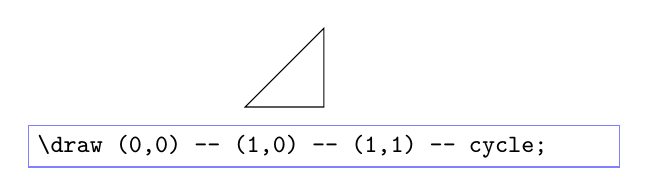
\begin{tikzpicture}
\draw (0,0) -- (1,0) -- (1,1) -- cycle;
\node[rectangle,draw=blue!50] at (1,-0.5) {
\begin{minipage}{0.6\textwidth}
\begin{verbatim}
\draw (0,0) -- (1,0) -- (1,1) -- cycle;
\end{verbatim}
\end{minipage}
};
\end{tikzpicture}
\end{center}

\subsection{Advanced}
\subsubsection{Style}
With \verb".style", we can define many kinds of nodes.
\begin{verbatim}
Cnode/.style={circle, draw=blue!50, fill=blue!20, very thick, minimum size=10mm},
\end{verbatim}
\verb"draw" is the color of frame, 50 and 20 are the depth of the color,
\verb"very thick" is the thickness of the frame. The shape can be
\verb"rectangle" or others.
After declaring the style, use \verb"\node[Cnode]" to use.
Line's shape can be adjusted as well. And you can put these \verb"style"
in \verb"\tikzset" outside the \verb"document" if you like.

\subsubsection{Function}
TikZ can plot function 
\begin{center}
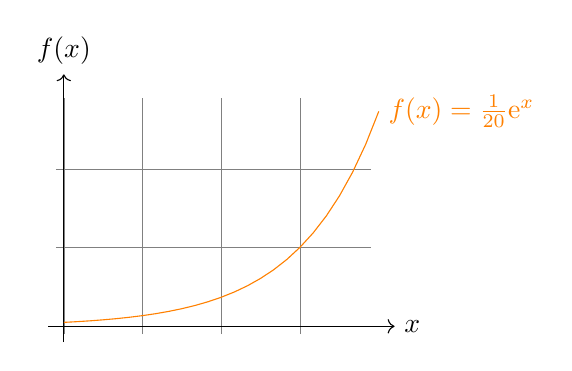
\begin{tikzpicture}[domain=0:4]
  \draw[very thin,color=gray] (-0.1,-0.1) grid (3.9,2.9);
  \draw[->] (-0.2,0) -- (4.2,0) node[right] {$x$};
  \draw[->] (0,-0.2) -- (0,3.2) node[above] {$f(x)$};
  \draw[color=orange] plot (\x,{0.05*exp(\x)}) node[right] {$f(x) = \frac{1}{20} \mathrm e^x$};
\end{tikzpicture}
\end{center}
with
\begin{center}
\begin{verbatim}
\begin{tikzpicture}[domain=0:4]
  \draw[very thin,color=gray] (-0.1,-1.1) grid (3.9,3.9);
  \draw[->] (-0.2,0) -- (4.2,0) node[right] {$x$};
  \draw[->] (0,-1.2) -- (0,4.2) node[above] {$f(x)$};
  \draw[color=orange] plot (\x,{0.05*exp(\x)}) 
        node[right] {$f(x) = \frac{1}{20} \mathrm e^x$};
\end{tikzpicture}
\end{verbatim}
\end{center}
Load data from external file (see details in PGFPLOTS):
\begin{verbatim}
\tikz \draw plot[mark=x,smooth] file {sine-data.table};
\end{verbatim}

\subsubsection{Control}
To get a more twisted line, you may use Bezier curve.
\begin{center}
\begin{tikzpicture}
\draw[line width=10pt,scale=0.8] (0,0) .. controls (1,1) .. (4,0) 
    .. controls (5,0) and (5,1) .. (4,1) -- (4,2);
\draw[color=gray,scale=0.8] (0,0)--(1,1)--(4,0)--(5,0)--(5,1)--(4,1)--(4,2);
\node[rectangle,draw=blue!50] at (10,0) {
\begin{minipage}{0.65\textwidth}
\begin{verbatim}
\begin{tikzpicture}
\draw[line width=10pt] (0,0)..controls (1,1)..(4,0) 
..controls (5,0) and (5,1)..(4,1)..(4,2);
\draw[color=gray] (0,0)--(1,1)--(4,0)
--(5,0)--(5,1)--(4,1)--(4,2);
\end{tikzpicture}
\end{verbatim}
\end{minipage}
};
\end{tikzpicture}
\end{center}
There are at most two control points.

\subsubsection{Tree}
Usually we can create a tree with instructions like
\begin{verbatim}
\node (p) {1};
\node (q) [below left=of p] {2};
\node (r) [below right=of p] {3};
\node {s} [below=of r] {4};
\draw (p) to (q);
\draw (p) to (r);
\draw (r) to (s);
\end{verbatim}
But there is a simpler way:
\begin{verbatim}
\node {1}
    child {node {2}}
    child {node {3}
        chile {node {4}}
    };
\end{verbatim}
With \verb"\usetikzlibrary{graphs}", we can
\begin{verbatim}
\tikz \graph [grow down, branch right] {
    1 -> {2, 3 -> {4}}
};
\end{verbatim}
This can be employed in more than trees
\begin{center}
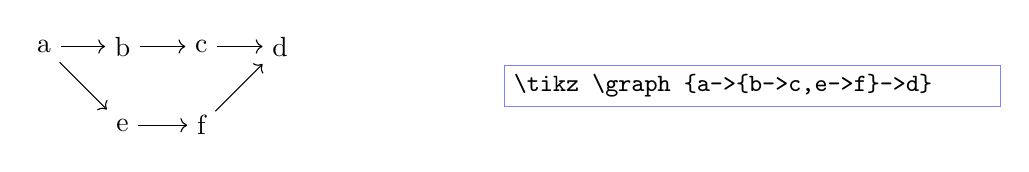
\begin{tikzpicture}
\graph{a->{b->c,e->f}->d;};
\node[rectangle,draw=blue!50] at (9,-0.5) {
\begin{minipage}{0.5\textwidth}
\begin{verbatim}
\tikz \graph {a->{b->c,e->f}->d}
\end{verbatim}
\end{minipage}
};
\end{tikzpicture}
\end{center}

\subsection{Commutative Diagrams}
Introduce the package \verb"tikz-cd".
\begin{center}
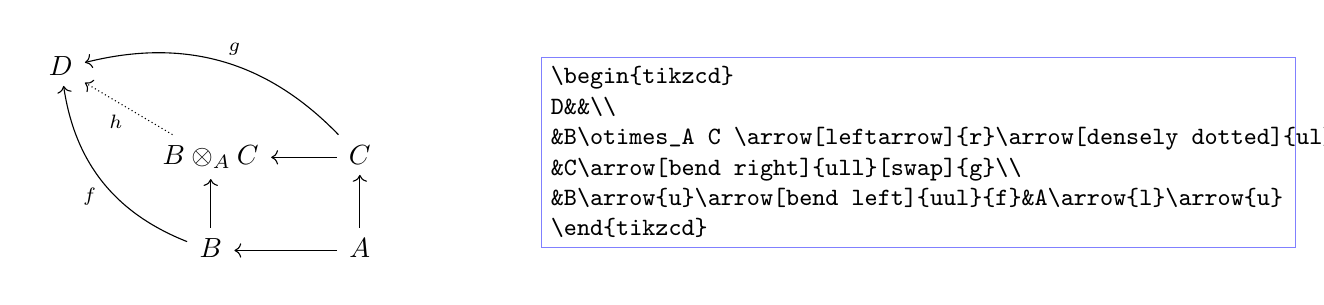
\begin{tikzpicture}
\node at (0,0) {
\begin{tikzcd}
D&&\\
&B\otimes_A C \arrow[leftarrow]{r}\arrow[densely dotted]{ul}{h}
&C\arrow[bend right]{ull}[swap]{g}\\
&B\arrow{u}\arrow[bend left]{uul}{f}&A\arrow{l}\arrow{u}
\end{tikzcd}};
\node[rectangle,draw=blue!50] at (9,0) {
\begin{minipage}{0.77\textwidth}
\begin{verbatim}
\begin{tikzcd}
D&&\\
&B\otimes_A C \arrow[leftarrow]{r}\arrow[densely dotted]{ul}{h}
&C\arrow[bend right]{ull}[swap]{g}\\
&B\arrow{u}\arrow[bend left]{uul}{f}&A\arrow{l}\arrow{u}
\end{tikzcd}
\end{verbatim}
\end{minipage}
};
\end{tikzpicture}
\end{center}
Items are arranged like matrix or tabular; Arrows
have the format 
\begin{verbatim}
\arrow[style]{relative position}{text}
\end{verbatim}

\subsubsection{Automaton}
\verb"\usetikzlibrary{automata}" This library contains several styles already 
define for your sake.
\begin{center}
\begin{tikzpicture}
\node at (0,0) {
\begin{tikzpicture}[node distance=2cm,auto]
\node[state,initial] (p) {a};
\node[state,accepting] (q) [above right of=p] {b};
\node[state] (r) [below right of=p] {c};
\path[->,thick,>=stealth] 
    (p) edge node {0} (q) edge node {1} (r)
    (r) edge node [right] {0} (q);
\end{tikzpicture}};
\node[rectangle,draw=blue!50] at (8.6,0) {
\begin{minipage}{0.63\textwidth}
\begin{verbatim}
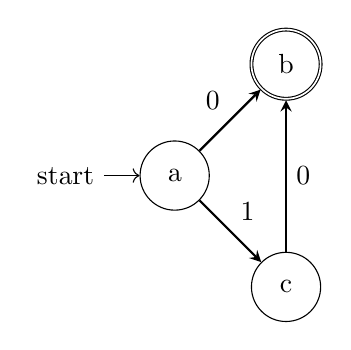
\begin{tikzpicture}[node distance=2cm,auto]
\node[state,initial] (p) {a};
\node[state,accepting] (q) [above right of=p] {b};
\node[state] (r) [below right of=p] {c};
\path[->,thick,>=stealth] 
(p) edge node {0} (q) edge node {1} (r)
(r) edge node [right] {0} (q);
\end{tikzpicture}
\end{verbatim}
\end{minipage}
};
\end{tikzpicture}
\end{center}

\subsubsection{Loop}
For graphs with largely repetitive pattern, TikZ provides loop method.
\begin{center}
\begin{tikzpicture}
\node at (0,0) {
\begin{tikzpicture}[scale=1.5]
\foreach \x in {18, 42,..., 360}
\node[circle,fill=black,scale=0.4] at (\x:1) {};
\foreach \x in {114, 138,...,450}
\foreach \y in {120, 144, 168}
\draw (\x:1)--(\x+\y:1);
\end{tikzpicture}};
\node[rectangle,draw=blue!50] at (8,0){
\begin{minipage}{0.6\textwidth}
\begin{verbatim}
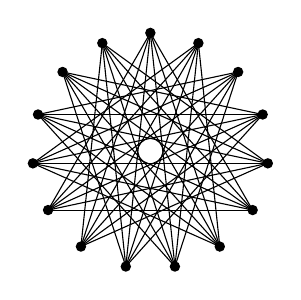
\begin{tikzpicture}[scale=1.5]
\foreach \x in {18, 42,..., 360}
\node[circle,fill=black,scale=0.4] at (\x:1) {};
\foreach \x in {114, 138,...,450}
\foreach \y in {120, 144, 168}
    \draw (\x:1)--(\x+\y:1);
\end{tikzpicture}
\end{verbatim}
\end{minipage}
};
\end{tikzpicture}
\end{center}
Note that the coordinate here is polar coordinate. The TikZ will find the pattern
of the omitted enumeration.\par
There is something more.
\begin{center}
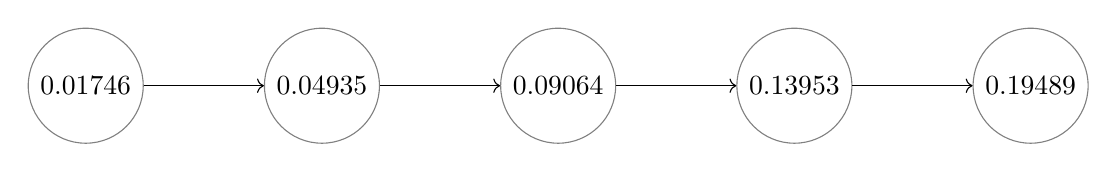
\begin{tikzpicture}
\foreach \x [count=\z,
    remember=\x as \pre,
    evaluate=\x as \y using sqrt(\x)*sin(\x),
    evaluate=\x as \p using \x*3] in {1,2,...,5}{
    \node[circle,draw=black!50] (c\x) at (\p,0) {$\y$};
    \ifnum \z>1
        \draw[->] (c\pre) to (c\x);
    \fi
}
\end{tikzpicture}
\end{center}
\begin{verbatim}
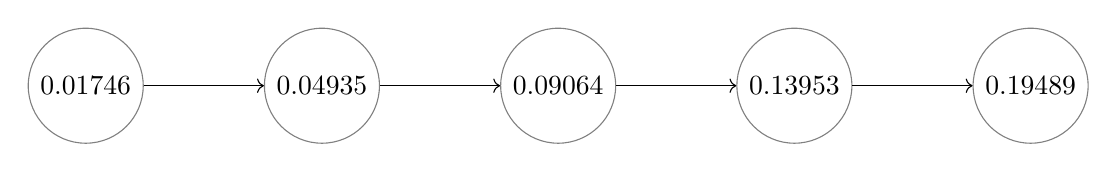
\begin{tikzpicture}
\foreach \x [count=\z,
    remember=\x as \pre,
    evaluate=\x as \y using sqrt(\x)*sin(\x),
    evaluate=\x as \p using \x*3] in {1,2,...,5}{
    \node[circle,draw=black!50] (c\x) at (\p,0) {$\y$};
    \ifnum \z>1
        \draw[->] (c\pre) to (c\x);
    \fi
}
\end{tikzpicture}
\end{verbatim}
You can use \verb"try" to draw different objects in loop.
\begin{center}

\begin{tikzpicture}[
    N1/.style={rectangle,fill=red!50},
    N2/.style={rectangle,fill=green!50},
    C/.style={circle,fill=blue!50},
]
\foreach \x [count=\z] in {1,2,C}
    \node[N\x/.try, \x/.try] at (\z,0) {}; 
\end{tikzpicture}
\end{center}
\begin{verbatim}

\begin{tikzpicture}[
    N1/.style={rectangle,fill=red!50},
    N2/.style={rectangle,fill=green!50},
    C/.style={circle,fill=blue!50},
]
\foreach \x [count=\z] in {1,2,C}
    \node[N\x/.try, \x/.try] at (\z,0) {}; 
\end{tikzpicture}
\end{verbatim}
Notice that if more than one is acceptable in \verb"try", latter ones will override 
former ones.

\subsection{Layout Design}
Use TikZ to design paper layout. It is easier to arrange figures and notations in
a more precise way.
But pay attention to some environment. They can not be directly in \verb"node";
you may need to specify the length of the environment by \verb"minipage".\par
This document's layout is organized by TikZ. 
See the raw code yourself for examples.

\section{Inkscape---Convert Painting to TikZ Code}
Inkscape is professional quality vector graphics software
which runs on Linux, Mac OS X and Windows desktop computers.
There are some key features:
\begin{enumerate}
    \item PSTricks export 
    \item TikZ export 
    \item Beamer drawing template
\end{enumerate}
The installation of TikZ export extension can be found 
\href{http://www.inkscapeforum.com/viewtopic.php?t=17898}{here}.\par
Also, there are other choices: \textit{tikzedt}, \textit{tikzit},
\textit{latexdraw}.\footnote{After trying all of them, I believe 
Inkscape is the most user-friendly.}\par
With the help of the GUI software, some difficult tasks can be 
easily accomplished. Also, it provides a way to convert .svg to
TikZ code, which means you can vectorize normal picture then 
export the TikZ code. An example for this is \href{https://tex.stackexchange.com/questions/60422/how-to-export-svg-to-tikz?noredirect=1&lq=1}{here}.


\section{Assignments}
There are two main parts of the assignments, one is mandatory and another is optional.
They are put separately in two folders under \textit{Week08-TikZ}.\par

You will compile those .tex's first to see the results, which are presented in 
\textit{standalone}. Then try to draw them by yourself.
Maybe you have a better way to draw some of the assignments;
please tell the others during the weekend discussion.

\end{document}
